\ifx\ucebnice\undefined
\documentclass[a4paper,10pt,oneside]{article}
\usepackage{latexsym}
\usepackage{amsmath}
\usepackage{amsfonts}
\usepackage{amsthm}
\usepackage{amssymb}
\usepackage{fncylab}
\usepackage{comment}
\usepackage{float}
\usepackage{wrapfig}
\usepackage{tikz}
\usepackage{tikz-qtree}
\usepackage{url}
\usepackage[bookmarks, colorlinks=false, 
            pdftitle={Úvod do programování --- Algoritmy},
            pdfauthor={Jonathan L. Verner}, 
            pdfsubject={Algoritmy a složitost}, 
            pdfkeywords={algoritmus, složitost, Python, třídění, grafy},
            bookmarksdepth=3
            ]{hyperref}
\usepackage[margin=1cm]{geometry}
\usetikzlibrary{decorations.fractals,chains,fit,shapes,patterns}
\usepackage[utf8]{inputenc}
\usepackage[T1]{fontenc}
\usepackage{attachfile}
\relpenalty=9999
\binoppenalty=9999


%----------definitions---------------------------


%math definitions

\newcommand{\R}{\mathbb R}
\newcommand{\C}{{\mathcal C}}
\newcommand{\F}{{{\mathcal F}}}
\newcommand{\U}{{{\mathcal U}}}
\newcommand{\V}{{{\mathcal V}}}
\newcommand{\cont}{{\mathfrak{c}}}
\newcommand{\force}{\Vdash}
\newcommand{\pw}{{{\mathcal P}}}
\newcommand{\MU}{{\mathbb{M}_{\mathcal{U}}}}
\newcommand{\pomega}{\pw(\omega)}


\newcommand{\src}[3]{%
\begin{program}%
\caption{#2\hfill%
\attachfile[author={Jonathan Verner},
            description={Source code for #2},
            mimetype={text/x-python},
            print=false,
            icon={Paperclip}]{kod/#1}}
\label{#3}\includecode[Python]{kod/#1}
\end{program}}


%---------numbering of the theorems------------
 \swapnumbers

 \newtheorem*{theorem*}{Theorem}
 \newtheorem{theorem}[subsection]{Theorem}
 \newtheorem{proposition}[subsection]{Proposition}
 \newtheorem{observation}[subsection]{Observation}
 \newtheorem{fact}[subsection]{Fact}
 \newtheorem{lemma}[subsection]{Lemma}
 \theoremstyle{definition}
 \newtheorem{definition}[subsection]{Definice}
 \newtheorem{question}[subsection]{Problém}
 \newtheorem{ukol}{Úloha}
 \newtheorem{cviceni}[subsection]{Cvičení}
 \newtheorem{cviceniH}[subsection]{Cvičení (*)}
 \newtheorem*{reseniIMPL*}{Řešení}
 \specialcomment{reseni}{\begin{reseniIMPL*}}{\end{reseniIMPL*}}
 \excludecomment{reseni}
 \excludecomment{todo}
 \newtheorem*{comments*}{Komentáře}
 \newtheorem*{definition*}{Definice}
 \newtheorem*{question*}{Question}
 \newtheorem{notation}[subsection]{Notation}
 \newtheorem{remark}[subsection]{Poznámka}
 \newtheorem{remark*}[subsection]{Poznámka}
 \newtheorem*{note}{Poznámka}
 \newtheorem*{ack}{Acknowledgements}
 \floatstyle{ruled}
 \newfloat{program}{htbp}{listings}[section]
 \floatname{program}{Algoritmus}
 
 \hypersetup{
    colorlinks,%
    citecolor=black,%
    filecolor=black,%
    linkcolor=black,%
    urlcolor=black
}
 
\pdfinfo{
      /Author (Jonathan Verner)
      /Title (ALG110006 Úvod do programování: Poznámky k přednášce, LS)
      /Subject (programování, algoritmy)
      /Keywords (quicksort,heapsort,dijsktra,graph,euclid)
   }
\include{pythonlisting}

\lstset{
numbers=left,
stepnumber=1,
numbersep=5pt,
numberstyle=\small\color{black}
}
%-------------opening--------------------------
\begin{document}
\title{}

% \author{Jonathan Verner}
% \address{Department of Logic, Charles University\\
% Palachovo nám. 2\\ 116 38 Praha 1, Czech Republic}
% \email{jonathan.verner{@}ff.cuni.cz}
%\thanks{The author was partially supported by }

%\subjclass[2010]{Primary }
%\keywords{}

%\begin{abstract}
%\end{abstract}
%\maketitle
\thispagestyle{empty}
\pagestyle{empty}
%\hsize=16cm
\parindent=0cm
\parskip=0.2cm

\setcounter{section}{2}
\fi
\section{Vyhledávání, třídící algoritmy}

\subsection*{Vyhledávání}\pdfbookmark[2]{Vyhledávání}{subsec:vyhledavani}
Nechme zelináře zelinářem a pojďme se spolu podívat na jinou úlohu. Tentokrát budeme chtít napsat spellchecker. Pro začátek bude
velmi jednoduchý. Dostane textový dokument a slovník a vypíše všechna slova, která se vyskytují v dokumentu a nevyskytují se
ve slovníku. V Pythonu to naprogramujeme velmi jednoduše:

\begin{python}
# Vrátí seznam všech slov nacházejících se ve stringu doc,
# která nejsou v seznamu slovnik. Předpokládáme že jednotlivá
# slova ve stringu doc jsou oddělena mezerou.

def spell_check(slovnik,doc):
  spatna = []
  for slovo in doc.split(' '):
    if slovo not in slovnik:
      spatna.append(slovo)
  return spatna
\end{python}

Toto jednoduché řešení však má své mouchy. Jaká je jeho složitost? Funkce musí nejprve rozdělit řetězec doc na jednotlivá slova.
Python toto provede za nás funkcí split, ale při troše dobré vůle bychom to zvládli sami a zjistili bychom, že složitost této
operace je $O(N)$, kde $N$ je délka řetězce. Pokud by nás zajímala složitost v závislosti na počtu slov, stačí si uvědomit, že
většina slov je kratších než nějakých 15 znaků a pravděpodobně žádné slovo nebude delší než 30 znaků. Z toho plyne, že složitost
bude opět $O(N)$ --- multiplikativní konstanty v $O$-notaci zanedbáváme. Pak musíme projít všechna slova a u každého otestovat,
zda se nachází ve slovníku. Ve výše uvedeném programu to za nás dělá operátor {\tt in}. Ten je v podstatě jen zkratkou
následujícího kódu:

\begin{python}
# Vrátí true, pokud se slovo vyskytuje v seznamu slovnik
def contains(slovo, slovnik):
  for s in slovnik:
    if s == slovo:
      return True
  return False
\end{python}

Z kódu je vidět, že složitost bude záviset na tom, jestli (a kde) se slovo {\tt slovo} ve slovníku {\tt slovnik} nachází. V ideálním
případě se {\tt slovo} nachází na prvním místě --- to provedeme pouze jednu operaci porovnání. V nejhorším případě v seznamu
nebude vůbec a pak provedeme tolik operací, kolik je prvků seznamu {\tt slovnik}. Složitost v nejhorším případě tedy bude $O(N+N*M) = O(N*M)$, kde
$N$ je počet slov ve vstupním dokumentu a $M$ je počet slov ve slovníku. Ukážeme si, že pokud věnujeme nějaký čas přípravě slovníku {\tt slovnik},
podaří se nám navrhnout funkci {\tt contains} tak, aby měla složitost $O(\log M)$, což dá pro celý algoritmus složitost $O(N*\log M)$.
Trik spočívá v tom, že si slovník předem uspořádáme podle abecedy. Jak to udělat uvidíme v další části, teď však předpokládejme, že
ho máme uspořádaný. K testu, zda se ve slovníku dané slovo nachází, teď můžeme využít metodu půlení intervalů --- vezmeme si
slovo uprostřed našeho slovníku a porovnáme ho s hledaným slovem. Pokud je v abecedě hledané slovo dříve, víme, že se musí
nacházet v první polovině slovníku. Pokud je naopak později, nachází se v druhé polovině. Ten samý postup budeme opakovat znovu,
dokud slovo buď nenajdeme, nebo nezjistíme, že ve slovníku není. Takto popsaný algoritmus nejlépe zapíšeme pomocí rekurze:

\begin{program}\caption{Binární vyhledávání}
\begin{python}
# Vrátí True, pokud se slovo vyskytuje v setřízeném
# seznamu slovnik[start:end]. Jinak vrátí False.
def contains(slovo, slovnik, start, end):
  if start >= end:
    return False
  middle = start + (end-start)/2
  if slovo == slovnik[middle]:
    return True
  elif slovo < slovnik[middle]:
    return contains(slovo, slovnik, start, middle)
  elif slovo > slovnik[middle]:
    return contains(slovo, middle+1, end)
\end{python}
\end{program}

Pojďme se nejprve přesvědčit, že algoritmus je správný. Jak je u rekurzivních algoritmů obvyklé, budeme postupovat indukcí, v tomto případě dle {\tt n=end-start}.
\begin{itemize}
 \item[{\tt n=0}] Pokud je {\tt start == end}, pak algoritmus vrátí False, což je správně, protože {\tt slovnik[start:start]} je prázdný seznam ve kterém se nic nevyskytuje.
 \item[{\tt n=1}] Pokud je {\tt end-start == 1}, pak {\tt middle == start} a {\tt slovnik[start:end] = [slovnik[start]]}. Pokud je tedy {\tt slovo == slovnik[middle]}, algoritmus
vrátí {\tt True}, jinak se tam slovo nevyskytuje. Pokud se tam nevyskytuje, zavolá se buď {\tt contains(slovo, slovnik, start, start)} nebo {\tt contains(slovo, slovnik, end,end)} což obojí
správně vrátí {\tt False}.
 \item[{\tt n+1}] Indukční krok. Předpokládejme že pro {\tt end-start = n >= 1 } algoritmus pracuje a uvažujme {\tt end-start = n+1}. Je jasné, že
pokud se slovo v seznamu {\tt slovnik[start:end]} vyskytuje, pak je buď rovno
\begin{center}
{\tt slovnik[middle]}
\end{center}
nebo se vyskytuje v
\begin{center}
{\tt slovnik[start:middle]}
\end{center}
nebo v
\begin{center}
{\tt slovnik[middle+1:end]}.
\end{center}
První případ je jasný a na druhé dva můžeme použít indukční předpoklad, protože jak
\begin{center}
{\tt middle-start < end-start}
\end{center}
tak
\begin{center}
{\tt end-(middle+1) < end-start}
\end{center}
(první případ plyne z toho, že {\tt start-end >= n+1>=2}).
\end{itemize}

A jaká je složitost algoritmu? Protože v každém kroku provedeme maximálně tři porovnání a jedno přiřazení a zároveň zmenšíme rozdíl {\tt end-start} na polovinu,
je intuitivně vcelku jasné, že složitost bude $4\log M = O(\log M)$.

\begin{cviceni} Indukcí dokažte, že složitost výše uvedené funkce {\tt contains} bude opravdu $O(\log M)$.
\end{cviceni}
\begin{reseni} ...
\end{reseni}

Máme tedy mnohem efektivnější funkci {\tt contains}, ale není to zadarmo. Aby tato funkce fungovala, je třeba mít slovník setřízený podle abecedy, což bude naším dalším tématem.
Předem můžeme prozradit, že složitost třídění bude $O(M\log M)$. Když se vrátíme k naší funkci {\tt spell\_check} dostaneme složitost $O((M+N)\log M)$. Jak to porovnat
s původní složitostí $O(N*M)$? V typickém případě bude slovník mnohem větší než seznam slov, tedy $M>>N$. Pokud například $N<\log M$ zjistíme, že původní algoritmus
bude lepší --- vzhledem k tomu, že budeme hledat jen pár slov, nevyplatí se nám třídit celý slovník. Na druhou stranu, pokud předpokládáme, že funkci {\tt spell\_check}
budeme využívat často (což je rozumný předpoklad), setřízení slovníku se nám dlouhodobě vyplatí.

\subsection*{Třídící algoritmy}\pdfbookmark[2]{Třídící algoritmy}{subsec:tridicialgoritmy}
\paragraph{Insertion Sort.}\pdfbookmark[3]{Insertion Sort}{par:insertionsort}
V předchozí části jsme narazili na úlohu setřídit seznam slov dle abecedy. Pojďme se zamyslet nad tím, jak bychom to mohli udělat. Jako první nás asi napadne postupovat
tak, jak bychom sami postupovali, pokud bychom měli úlohu vyřešit ručně. Prostě bychom si setřízený seznam budovali postupně a v každém kroku do již setřízené části
zatřídili další slovo. Tomuto algoritmu se říká \emph{insertion sort}. Zapišme si ho v Pythonu:

\src{insertionsort}{Insertion Sort}

V proměnné {\tt last\_sorted} si algoritmus udržuje index posledního setřízeného prvku (t.j. pole {\tt seznam[:last\_sorted+1]} je setřízené).
Na začátku je setřízený pouze první prvek pole (řádek 2). Dokud není pole setřízené celé (podmínka na řádku 3), provádím následující kroky (řádky 4-8):
vezmu první nesetřízený prvek (řádek 4), zatřídím ho do pole na správné místo (řádky 5-7) a zvětším si index posledního setřízeného prvku (řádek 8).

Jaká je složitost tohoto algoritmu? Cyklus na řádku 3 se provede $n$-krát, kde $n$ je velikost vstupního pole {\tt seznam}. V těle cyklu pak provedu
dvě přiřazovací operace (řádky 4, 8) a zatřízení (cyklus na řádcích 5-7). Vnitřní zatřizovací cyklus provede v nejhorším případě $3\cdot {\tt j}$ operací.
Po chvilce počítání (je třeba sečíst řadu $1 + 2 + \cdots + n$) dostanu celkový dolní odhad složitosti $2n + 3n(n+1)/2 = O(n^2)$.

\begin{cviceni} Jaká bude složitost algoritmu, pokud ho pustíme na již setřízené pole?
\end{cviceni}

Za chvíli uvidíme, že existují algoritmy s mnohem lepší asymptotickou složitostí. Proč jsme tedy insertion sort vůbec zmiňovali? Kromě toho, že
je to algoritmus velmi jednoduchý, má několik podstatných výhod. Ačkoliv je jeho \emph{asymptotická} složitost kvadratická, pro malá vstupní pole
(do velikosti cca 100 prvků) je často nejrychlejším algoritmem. Další výhodou je jeho optimální chování, pokud ho pustíme na již setřízené pole
(viz cvičení). Další možnou výhodou je to, že pole zpracovává postupně --- algoritmy, které popíšeme dále, potřebují znát pole celé najednou.

\paragraph{Heap sort.}\pdfbookmark[3]{Heap Sort}{par:heapsort} Pokud vám prozradím, že optimální asymptotická složitost třídících algoritmů (založených na provnávání prvků) je $O(n\log n)$
a navíc Vám napovím, že lze použít haldu, možná Vás už napadne, jak funguje algoritmus, kterému se říká \emph{heap sort}. Vzpomeňte si, že
operace přidání prvku do haldy ({\tt push}) a odebrání nejmenšího prvku z haldy ({\tt pop}) má složitost $O(\log n)$. Co kdybychom postupně
prošli celé pole a každý prvek přidali na haldu a pak postupně odebírali vždy nejmenší prvek z haldy? To je princip heap sortu (viz výpis \ref{alg:heapsort})

\begin{program}\caption{Heap sort}\label{alg:heapsort}
\begin{python}
def heap_sort(seznam):
  halda = []
  for p in seznam:
    push(halda, p)

  for i in range(len(seznam)):
    p = pop(halda)
    seznam[i] = p
\end{python}
\end{program}

Kód uvedený ve výpisu \ref{alg:heapsort} je pěkný (a není těžké spočítat, že má asymptotickou složitost $O(n\log n)$\footnote{Tak, jak je napsaný, má první cyklus, který staví haldu,
složitost $O(n\log n)$. Dá se však napsat trochu chytřeji tak, aby měl složitost lineární (viz např. \cite{Wirth:1985}). Druhý cyklus se takto
přepsat nedá, složitost tedy bude stále $O(n\log n)$}), není však moc efektivní --- k setřízení pole si
v paměti vyhradí ještě jednou tolik místa na haldu, na kterou postupně přidává prvky. Tento nedostatek však lze velmi jednoduše odstranit.
Když se nad tím zamyslíte a uvědomíte si, že jednoprvkové pole je haldou, určitě pro Vás následující cvičení nebude příliš obtížné:

\begin{cviceni} Přepište heap sort (a haldové operace {\tt push} resp. {\tt push}) tak, aby algoritmus nepotřeboval separátní seznam pro haldu.
\end{cviceni}

Další algoritmus, který si ukážeme, je asi v praxi nejpoužívanějším algoritmem.

\paragraph{Quicksort}\pdfbookmark[3]{Quicksort}{par:quicksort} je klasickým rekurzivním algoritmem. Funguje na
následujícím principu. Pokud seznam, který se má setřídit, má pouze jeden prvek, je setřízený a algoritmus
může skončit. V opačném případě si seznam rozdělí na dvě části tak, aby všechny položky v levé části byly
menší než všechny položky v pravé části. Pak se rekurzivně zavolá a setřídí
levou a pravou část. Následně může prostě připojit setřízenou pravou část za setřízenou levou část
a celý seznam bude setřízený, protože prvky vlevo byly menší než prvky vpravo a obě části setřízené
byly. Zbývá popsat rozdělování na části. To se typicky provádí tak, že se ze seznamu náhodně zvolí jeden
prvek, tzv. \emph{pivot}, a pole se rozdělí tak, aby vlevo byly všechny prvky menší nebo rovné pivotu
a vpravo všechny prvky větší nebo rovné pivotu. Seznamem se prochází současně zleva i zprava. V okamžiku, kdy z
jednoho směru narazíme na prvek, který má být vzhledem k pivotu v opačné části, čekáme, než k takovému
prvku dorazíme i zprava (pokud na žádný nenarazíme, víme, že jsme hotovi a tento prvek bude první prvek,
který patří do pravé části). V okamžiku, kdy na takový prvek narazíme i zprava, oba prvky vyměníme
a pokračujeme. Když se setkáme, máme pole rozdělené. Schematicky bude quicksort vypadat takto:

\begin{python}
def quicksort( seznam ):
    if len(seznam) == 1:
      return seznam
    pivot = zvol_pivota( seznam )
    L, P = rozdel_seznam( seznam, pivot )
    L_sorted = quicksort(L)
    P_sorted = quicksort(P)
    return L_sorted + P_sorted
\end{python}

\begin{remark} Ve skutečnosti by výše uvedený schematicky zapsaný quicksort byl relativně pomalý,
protože by docházelo k častému kopírování z paměti do paměti při vytváření nových polí (L,P, L+P).
V reálu proto vůbec nebudeme vytvářet nové seznamy a funkce quicksort bude vypadat spíše tak, jak je uvedena ve výpisu \ref{alg:quicksort}.

\begin{program}\caption{Quicksort}\label{alg:quicksort}
\begin{python}
def quicksort( seznam, start, end ):
    if start >= end:
        # Prazdné a jednoprvkové pole jsou
        # z definice setřízené
        return
    pivot = zvol_pivota( seznam, start, end )
    stred = rozdel_seznam( seznam, start, end, pivot)
    quicksort( seznam, start, stred )
    quicksort( seznam, stred+1, end )
    return
\end{python}
\end{program}

t.j. všechno se bude odehrávat v poli {\tt seznam}, nic se nebude nikam kopírovat a podseznamy budou
vždy vymezené dvěma indexy, počátečním ({\tt start}) a koncovým ({\tt end}).
\end{remark}

\begin{remark} Při rozdělování pole je třeba dát pozor na to, aby se pole opravdu ``rozdělilo'', t.j.
aby bylo {\tt start <= stred < end}. Pokud by totiž pravá nebo levá část byla prázdná, program
by se zacyklil. Tuto podmínku nicméně není těžké splnit, protože pivot může být prvkem jak pravé,
tak levé části.
\end{remark}

\begin{cviceni} Naprogramujte funkce {\tt zvol\_pivota} a {\tt rozdel\_seznam}!
\end{cviceni}

Jaká je složitost quicksortu? V optimálním případě, pokud by se nám vždy povedlo zvolit pivota tak, aby levá i pravá část
pole byla stejně velká, by byla složitost $O(n\log n)$. Pěkně to lze nahlédnout na následujícím obrázku, kde červená políčka
odpovídají levým částem pole, žlutá pravým. Čísla pod polem pak udávají, kolik operací musím provést při dělení daného pole:
\begin{center}
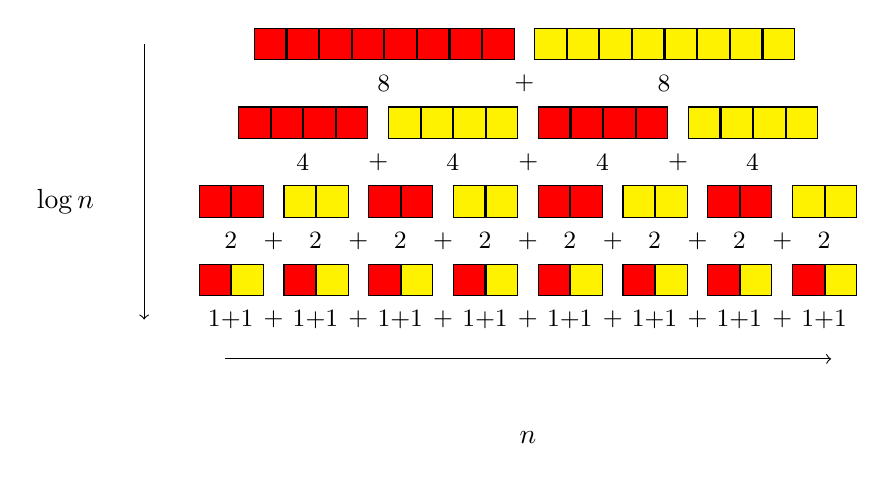
\begin{tikzpicture}
\tikzstyle{free}=[minimum size=0.1cm]
\tikzstyle{sfree}=[minimum size=0.05cm]
\tikzstyle{l}=[draw,minimum size=0.4cm,fill=red]
\tikzstyle{r}=[draw,minimum size=0.4cm,fill=yellow]
\begin{scope}[start chain=1 going right,node distance=0mm,shift={(2cm,2cm)}]
    \node [on chain=1,l] {\tiny };
    \node [on chain=1,l] {\tiny };
    \node [on chain=1,l] {\tiny };
    \node [on chain=1,l] (start1) {\tiny };
    \node [on chain=1,l] {\tiny };
    \node [on chain=1,l] {\tiny };
    \node [on chain=1,l] {\tiny };
    \node [on chain=1,l] {\tiny };
    \node [on chain=1,free] (center1) {\tiny };
    \node [on chain=1,r] {\tiny};
    \node [on chain=1,r] {\tiny };
    \node [on chain=1,r] {\tiny };
    \node [on chain=1,r] (start2) {\tiny };
    \node [on chain=1,r] {\tiny };
    \node [on chain=1,r] {\tiny };
    \node [on chain=1,r] {\tiny };
    \node [on chain=1,r] {\tiny };
    \node [node distance=0.5cm,below of=start1, shift={(0.2cm,0cm)}] {\small 8};
    \node [node distance=0.5cm,below of=center1] {\small +};
    \node [node distance=0.5cm,below of=start2, shift={(0.2cm,0cm)}] {\small 8};
\end{scope}

\begin{scope}[start chain=1 going right,node distance=0mm,shift={(1.8cm,1cm)}]
    \node [on chain=1,l] {\tiny };
    \node [on chain=1,l] (start1) {\tiny };
    \node [on chain=1,l] {\tiny };
    \node [on chain=1,l] {\tiny };
    \node [on chain=1,free] (center1) {\tiny };
    \node [on chain=1,r] {\tiny };
    \node [on chain=1,r] (start2) {\tiny };
    \node [on chain=1,r] {\tiny };
    \node [on chain=1,r] {\tiny };
    \node [on chain=1,free] (center2) {\tiny };
    \node [on chain=1,l] {\tiny};
    \node [on chain=1,l] (start3) {\tiny };
    \node [on chain=1,l] {\tiny };
    \node [on chain=1,l] {\tiny };
    \node [on chain=1,free] (center3) {\tiny };
    \node [on chain=1,r] {\tiny };
    \node [on chain=1,r] (start4) {\tiny };
    \node [on chain=1,r] {\tiny };
    \node [on chain=1,r] {\tiny };
    \node [node distance=0.5cm,below of=start1, shift={(0.2cm,0cm)}] {\small 4};
    \node [node distance=0.5cm,below of=center1] {\small +};
    \node [node distance=0.5cm,below of=start2, shift={(0.2cm,0cm)}] {\small 4};
    \node [node distance=0.5cm,below of=center2] {\small +};
    \node [node distance=0.5cm,below of=start3, shift={(0.2cm,0cm)}] {\small 4};
    \node [node distance=0.5cm,below of=center3] {\small +};
    \node [node distance=0.5cm,below of=start4, shift={(0.2cm,0cm)}] {\small 4};
\end{scope}

\begin{scope}[start chain=1 going right,node distance=0mm,shift={(1.3cm,0cm)}]
    \node [on chain=1,l] (start1) {\tiny };
    \node [on chain=1,l] {\tiny };
    \node [on chain=1,sfree] (center1) {\tiny };
    \node [on chain=1,r] (start2) {\tiny };
    \node [on chain=1,r] {\tiny };
    \node [on chain=1,sfree] (center2) {\tiny };
    \node [on chain=1,l] (start3) {\tiny };
    \node [on chain=1,l] {\tiny };
    \node [on chain=1,sfree] (center3) {\tiny };
    \node [on chain=1,r] (start4) {\tiny };
    \node [on chain=1,r] {\tiny };
    \node [on chain=1,sfree] (center4) {\tiny };
    \node [on chain=1,l] (start5) {\tiny};
    \node [on chain=1,l] {\tiny };
    \node [on chain=1,sfree] (center5) {\tiny };
    \node [on chain=1,r] (start6) {\tiny };
    \node [on chain=1,r] {\tiny };
    \node [on chain=1,sfree] (center6) {\tiny };
    \node [on chain=1,l] (start7) {\tiny };
    \node [on chain=1,l] {\tiny };
    \node [on chain=1,sfree] (center7) {\tiny };
    \node [on chain=1,r] (start8) {\tiny };
    \node [on chain=1,r] {\tiny };
    \node [node distance=0.5cm,below of=start1, shift={(0.2cm,0cm)}] {\small 2};
    \node [node distance=0.5cm,below of=center1] {\small +};
    \node [node distance=0.5cm,below of=start2, shift={(0.2cm,0cm)}] {\small 2};
    \node [node distance=0.5cm,below of=center2] {\small +};
    \node [node distance=0.5cm,below of=start3, shift={(0.2cm,0cm)}] {\small 2};
    \node [node distance=0.5cm,below of=center3] {\small +};
    \node [node distance=0.5cm,below of=start4, shift={(0.2cm,0cm)}] {\small 2};
    \node [node distance=0.5cm,below of=center4] {\small +};
    \node [node distance=0.5cm,below of=start5, shift={(0.2cm,0cm)}] {\small 2};
    \node [node distance=0.5cm,below of=center5] {\small +};
    \node [node distance=0.5cm,below of=start6, shift={(0.2cm,0cm)}] {\small 2};
    \node [node distance=0.5cm,below of=center6] {\small +};
    \node [node distance=0.5cm,below of=start7, shift={(0.2cm,0cm)}] {\small 2};
    \node [node distance=0.5cm,below of=center7] {\small +};
    \node [node distance=0.5cm,below of=start8, shift={(0.2cm,0cm)}] {\small 2};
\end{scope}

\begin{scope}[start chain=1 going right,node distance=0mm,shift={(1.3cm,-1cm)}]
    \node [on chain=1,l] (start1) {\tiny };
    \node [on chain=1,r] (start2) {\tiny };
    \node [on chain=1,sfree] (center1) {\tiny };
    \node [on chain=1,l] (start3) {\tiny };
    \node [on chain=1,r] (start4) {\tiny };
    \node [on chain=1,sfree] (center2) {\tiny };
    \node [on chain=1,l] (start5) {\tiny };
    \node [on chain=1,r] (start6) {\tiny };
    \node [on chain=1,sfree] (center3) {\tiny };
    \node [on chain=1,l] (start7) {\tiny };
    \node [on chain=1,r] (start8) {\tiny };
    \node [on chain=1,sfree] (center4) {\tiny };
    \node [on chain=1,l] (start9) {\tiny};
    \node [on chain=1,r] (start10) {\tiny };
    \node [on chain=1,sfree] (center5) {\tiny };
    \node [on chain=1,l] (start11) {\tiny };
    \node [on chain=1,r] (start12) {\tiny };
    \node [on chain=1,sfree] (center6) {\tiny };
    \node [on chain=1,l] (start13) {\tiny };
    \node [on chain=1,r] (start14) {\tiny };
    \node [on chain=1,sfree] (center7) {\tiny };
    \node [on chain=1,l] (start15) {\tiny };
    \node [on chain=1,r] (start16) {\tiny };
    \node [node distance=0.5cm,below of=start1, shift={(0.2cm,0cm)}] {\small 1+1};
    \node [node distance=0.5cm,below of=center1] {\small +};
    \node [node distance=0.5cm,below of=start3, shift={(0.2cm,0cm)}] {\small 1+1};
    \node [node distance=0.5cm,below of=center2] {\small +};
    \node [node distance=0.5cm,below of=start5, shift={(0.2cm,0cm)}] {\small 1+1};
    \node [node distance=0.5cm,below of=center3] {\small +};
    \node [node distance=0.5cm,below of=start7, shift={(0.2cm,0cm)}] {\small 1+1};
    \node [node distance=0.5cm,below of=center4] {\small +};
    \node [node distance=0.5cm,below of=start9, shift={(0.2cm,0cm)}] {\small 1+1};
    \node [node distance=0.5cm,below of=center5] {\small +};
    \node [node distance=0.5cm,below of=start11, shift={(0.2cm,0cm)}] {\small 1+1};
    \node [node distance=0.5cm,below of=center6] {\small +};
    \node [node distance=0.5cm,below of=start13, shift={(0.2cm,0cm)}] {\small 1+1};
    \node [node distance=0.5cm,below of=center7] {\small +};
    \node [node distance=0.5cm,below of=start15, shift={(0.2cm,0cm)}] {\small 1+1};
    \node [node distance=1cm, below of=start1] (startL) {};
    \node [node distance=1cm, below of=start16] (endL) {};
    \node [node distance=2cm, below of=center4] {$n$};
    \draw[draw,->]
         (startL) -- (endL);
%     \draw[draw,->]
%       (end)..controls +(south:0.1) ..(endl);
%     \draw[dashed,->]
%       (end)..controls +(south:0.8) and +(north:0.9)..(endlone);
\end{scope}

\begin{scope}[shift={(0.4cm,0cm)}]
     \draw[draw,->] (0,2) -- (0,-1.5);
     \node [node distance=0cm, shift={(-1cm,0cm)}] (log) {$\log n$};
\end{scope}

\end{tikzpicture}
\end{center}

Formálně lze správnost odhadu ukázat například indukcí dle $n$ (pro jednoduchost uvažujeme pouze pole velikosti $n=2^k$): Pro pole velikosti $2^0$ je to zřejmé.
Mám-li nyní dáno pole velikosti $2^k$, musím  rozdělit pole (složitost $2^k$) a dvakrát zavolat quicksort na pole
poloviční velikosti. Z indukčního předpokladu má jedno takové volání složitost $2^{(k-1)}\log 2^{(k-1)}) = 2^{k-1}(k-1)$, dvě volání tedy budou mít složitost
$2^k(k-1)$. Celkem tedy $2^k + 2^k(k-1) = 2^k k = O(2^k k) = O(n\log n)$.

Jaká bude složitost quicksortu, pokud se nám pivoty nepodaří zvolit optimálně? Představme si, že jako pivota volím vždy první prvek pole a na vstupu dostanu
pole již setřízené. Co se stane je opět dobře vidět na obrázku:

\begin{center}
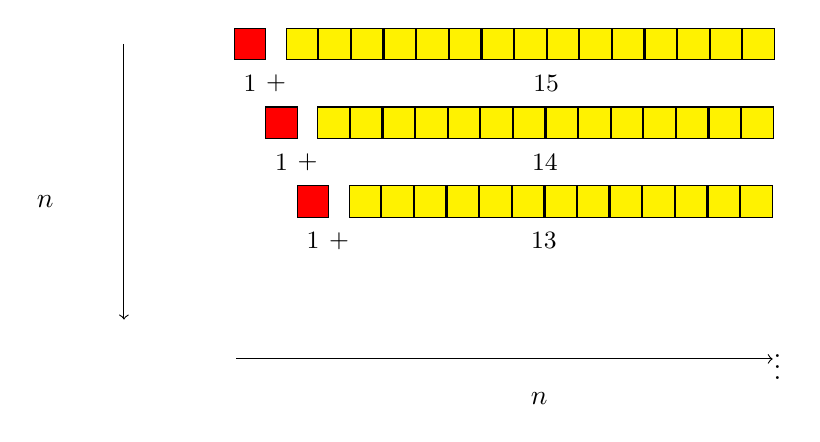
\begin{tikzpicture}
\tikzstyle{free}=[minimum size=0.1cm]
\tikzstyle{sfree}=[minimum size=0.05cm]
\tikzstyle{l}=[draw,minimum size=0.4cm,fill=red]
\tikzstyle{r}=[draw,minimum size=0.4cm,fill=yellow]
\begin{scope}[start chain=1 going right,node distance=0mm,shift={(2cm,2cm)}]
    \node [on chain=1,l] (start1) {\tiny };
    \node [on chain=1,free] (center1) {\tiny };
    \node [on chain=1,r] {\tiny };
    \node [on chain=1,r] {\tiny };
    \node [on chain=1,r] {\tiny };
    \node [on chain=1,r] {\tiny };
    \node [on chain=1,r] {\tiny };
    \node [on chain=1,r] {\tiny };
    \node [on chain=1,r] {\tiny };
    \node [on chain=1,r] (start2) {\tiny};
    \node [on chain=1,r] {\tiny };
    \node [on chain=1,r] {\tiny };
    \node [on chain=1,r] {\tiny };
    \node [on chain=1,r] {\tiny };
    \node [on chain=1,r] {\tiny };
    \node [on chain=1,r] {\tiny };
    \node [on chain=1,r] {\tiny };
    \node [node distance=0.5cm,below of=start1, shift={(0cm,0cm)}] {\small 1};
    \node [node distance=0.5cm,below of=center1] {\small +};
    \node [node distance=0.5cm,below of=start2, shift={(0.2cm,0cm)}] {\small 15};
\end{scope}
\begin{scope}[start chain=1 going right,node distance=0mm,shift={(2.4cm,1cm)}]
    \node [on chain=1,l] (start1) {\tiny };
    \node [on chain=1,free] (center1) {\tiny };
    \node [on chain=1,r] {\tiny };
    \node [on chain=1,r] {\tiny };
    \node [on chain=1,r] {\tiny };
    \node [on chain=1,r] {\tiny };
    \node [on chain=1,r] {\tiny };
    \node [on chain=1,r] {\tiny };
    \node [on chain=1,r] (start2) {\tiny};
    \node [on chain=1,r] {\tiny };
    \node [on chain=1,r] {\tiny };
    \node [on chain=1,r] {\tiny };
    \node [on chain=1,r] {\tiny };
    \node [on chain=1,r] {\tiny };
    \node [on chain=1,r] {\tiny };
    \node [on chain=1,r] {\tiny };
    \node [node distance=0.5cm,below of=start1, shift={(0cm,0cm)}] {\small 1};
    \node [node distance=0.5cm,below of=center1] {\small +};
    \node [node distance=0.5cm,below of=start2, shift={(0.2cm,0cm)}] {\small 14};
\end{scope}

\begin{scope}[start chain=1 going right,node distance=0mm,shift={(2.8cm,0cm)}]
    \node [on chain=1,l] (start1) {\tiny };
    \node [on chain=1,free] (center1) {\tiny };
    \node [on chain=1,r] {\tiny };
    \node [on chain=1,r] {\tiny };
    \node [on chain=1,r] {\tiny };
    \node [on chain=1,r] {\tiny };
    \node [on chain=1,r] {\tiny };
    \node [on chain=1,r] (start2) {\tiny };
    \node [on chain=1,r] {\tiny};
    \node [on chain=1,r] {\tiny };
    \node [on chain=1,r] {\tiny };
    \node [on chain=1,r] {\tiny };
    \node [on chain=1,r] {\tiny };
    \node [on chain=1,r] {\tiny };
    \node [on chain=1,r] {\tiny };
    \node [node distance=0.5cm,below of=start1, shift={(0cm,0cm)}] {\small 1};
    \node [node distance=0.5cm,below of=center1] {\small +};
    \node [node distance=0.5cm,below of=start2, shift={(0.2cm,0cm)}] {\small 13};
\end{scope}
\begin{scope}[start chain=1 going right, node distance=0mm,shift={(3cm,-1cm)}]
 \node[node distance=0.5cm,shift={(5.7cm,-1cm)}] (log) {$\vdots$};
\end{scope}



\begin{scope}[start chain=1 going right,node distance=0mm,shift={(1.7cm,-1cm)}]
    \node [on chain=1,free] (start1) {\tiny };
    \node [on chain=1,free] (start2) {\tiny };
    \node [on chain=1,sfree] (center1) {\tiny };
    \node [on chain=1,free] (start3) {\tiny };
    \node [on chain=1,free] (start4) {\tiny };
    \node [on chain=1,sfree] (center2) {\tiny };
    \node [on chain=1,free] (start5) {\tiny };
    \node [on chain=1,free] (start6) {\tiny };
    \node [on chain=1,sfree] (center3) {\tiny };
    \node [on chain=1,free] (start7) {\tiny };
    \node [on chain=1,free] (start8) {\tiny };
    \node [on chain=1,sfree] (center4) {\tiny };
    \node [on chain=1,free] (start9) {\tiny};
    \node [on chain=1,free] (start10) {\tiny };
    \node [on chain=1,sfree] (center5) {\tiny };
    \node [on chain=1,free] (start11) {\tiny };
    \node [on chain=1,free] (start12) {\tiny };
    \node [on chain=1,sfree] (center6) {\tiny };
    \node [on chain=1,free] (start13) {\tiny };
    \node [on chain=1,free] (start14) {\tiny };
    \node [on chain=1,sfree] (center7) {\tiny };
    \node [on chain=1,free] (start15) {\tiny };
    \node [on chain=1,free] (start16) {\tiny };
    \node [node distance=1cm, below of=start1] (startL) {};
    \node [node distance=1cm, below of=start16, shift={(1.6cm,0cm)}] (endL) {};
    \node [node distance=1.5cm, below of=start12] {$n$};
    \draw[draw,->]
         (startL) -- (endL);
\end{scope}

\begin{scope}[shift={(0.4cm,0cm)}]
     \draw[draw,->] (0,2) -- (0,-1.5);
     \node[node distance=0cm,shift={(-1cm,0cm)}] (log) {$n$};
\end{scope}

\end{tikzpicture}
\end{center}

Na předchozím obrázku jsme měli úplný binární strom, jehož hloubka je $\log n$. Zde nám tento strom zdegeneroval ve strom, jehož hloubka je $n$. Když si spočteme
složitost, uvidíme, že je to $O(n^2)$, což je nepříjemné (tato situace by mohla nastat i v případě, že je pole již setřízené; v takovém případě
má i jednoduchý insertion sort složitost dokonce lineární!). Je tedy
vidět, že vhodná volba pivota může radikálně ovlivnit délku výpočtu. Jak jsme si ukázali výše, optimální volbou by byl medián pole. Protože
pro volbu mediánu existuje algoritmus běžící v lineárním čase (detaily viz \cite{BFPRT:1973}, nebo heslo {\tt Selection Algorithm} na \emph{Wikipedii}),
mohli bychom jej použít a zajistit si, že složitost quicksortu bude $O(n \log n)$ i v nejhorším případě. Nicméně v praktických implementacích se ukazuje, že
je rychlejší jako pivota zvolit nějaký náhodný prvek pole (nikoliv tedy vždy první!). Není tak sice zajišťeno, že algoritmus poběží v $O(n\log n)$, ale ve
většině případů poběží mnohem rychleji, než kdyby pivota vybíral složitěji\footnote{Navíc jsou implementace napsány tak, že pokud zjistí, že hrozí kvadratická
složitost --- například se pole několikrát po sobě rozdělilo velmi nerovnoměrně --- přepnou se třeba na heap sort, který je sice trochu pomalejší, ale má
garantovanou složitost $O(n\log n)$}.

Mohli bychom nyní pokračovat zkoumáním dalších třídících algoritmů a věnovat tomu ještě několik kapitol. Také bychom se mohli zabývat i jinými parametry
třídících algoritmů než jen jejich časovou složitostí --- mohli bychom například zkoumat jejich stabilitu nebo paměťovou náročnost. Zde to ale dělat
nebudeme a odkážeme zájemce do literatury. Místo toho se ještě chvíli budeme zabývat časovou složitostí a budou nás zajímat dolní odhady.

\subsection*{Dolní odhad pro složitost vyhledávání}\pdfbookmark[2]{Dolní odhad složitosti}{subsec:sortinglowerbound}

Ukázali jsme si, že algoritmus Quicksort má v optimálním čase složitost $O(n\log n)$. Algoritmus Heap sort má dokonce v nejhorším případě složitost $O(n\log n)$.
Podobně třeba algoritmus Merge sort (který jsme si neukazovali) má v nejhorším případě složitost $O(n\log n)$. Nemohli bychom najít nějaký ještě lepší algoritmus?
Ukážeme si, že pokud jako základní operace povolíme pouze porovnávat jednotlivé prvky případně je prohazovat, lepší algoritmy neexistují. Bude to však trochu složitější, než dokazovat, že nějaký algoritmus má takovou a takovou
složitost. Budeme totiž chtít ukázat, že žádný třídící algoritmus nemůže běžet rychleji než $O(n\log n)$\footnote{Formálně vzato následující úvaha dává dolní odhad pro složitost v \emph{nejhorším} případě. Malou úpravou bychom mohli ukázat, že odhad platí i pro složitost v \emph{průměrném případě}.} Jak takovou věc ukázat? Rozhodně nemůžeme procházet
třídící algoritmy jeden po druhém a dokazovat, že mají složitost nejméně $O(n\log n)$. Náš postup bude následující. Ukážeme, že máme-li nějaký rychlý algoritmus,
pak to nemůže být třídící algoritmus --- nalezneme pole, které nesetřídí správně. Představme si tedy, že máme nějaký algoritmus $A$, který na vstupu dostane
seznam čísel $x_0,\ldots,x_n$, která má setřídit. Pro jednoduchost budeme předpokládat, že výstupem bude posloupnost indexů $\mathbf{a}=(a_0,\ldots,a_n)$ setřízeného pole, t.j.
$a_0$ je index nejmenšího prvku, $a_1$ index druhého nejmenšího prvku a tak dále. Řekněme, že tento algoritmus má složitost $g(n)<O(n\log n)$. Při svém běhu
tedy může provést nejvýše $g(n)$ operací porovnání a každé takové porovnání má pouze dva možné výsledky \emph{menší}, \emph{větší} (rovnost pro jednoduchost zanedbáme).
Označíme-li si tedy tyto výsledky jako $0$ a $1$, dostaneme pro každý běh algoritmu posloupnost nul a jedniček $\mathbf{p}=(p_0,\ldots,p_{g(n)})$ délky (nejvýše) $g(n)$.
Množinu všech takových posloupností budeme značit $P(n)$. Ke každé posloupnosti nám algoritmus dá posloupnost indexů $\mathbf{a}$, což je prostá posloupnost čísel od $0$ do $n$.
Označme si množinu všech prostých posloupností čísel od $0$ do $n$ symbolem $A(n)$. Náš algoritmus nám tedy dává funkci $f:P(n)\to A(n)$.
Ukážeme, že pro dostatečně velká $n$ bude množina $A(n)$ větší než množina $P(n)$. To znamená, že bude existovat posloupnost $\mathbf{a}=(a_0, \ldots, a_n)\in A(n)$,
která nemá žádný vzor --- není výstupem algoritmu pro žádný vstup. Zvolíme tedy čísla $x_0,\ldots, x_n$ tak,
abychom jejich setřízením získali indexy $a_0, \ldots, a_n$. Pustíme na ně náš algoritmus, který začne čísla porovnávat --- tím získáme posloupnost $\mathbf{p}$.
Protože ale posloupnost $\mathbf{a}$ byla volená tak, aby nebyla výstupem algoritmu, algoritmus musí vrátit posloupnost jinou, která tudíž nebude správně
setřízená!

Zbývá tedy ukázat, že pro dostatečně velké $n$ bude množina $A(n)$ větší než množina $P(n)$. Spočíst velikost množiny $P(n)$ je jednoduché, je to
$2^0 + 2^1 + \cdots + 2^{g(n)-1} + 2^{g(n)} = 2^{g(n)+1}-1$. Velikost množiny $A(n)$ je $n!$. Protože se však s faktoriály špatně pracuje, uvědomme si, že
$n!>(n/2)^{n/2}$ --- to nám bude stačit. Protože algoritmus byl asymptoticky rychlejší než $O(n\log n) = O(n\log n - n)$, víme, že pro libovolné $K,b$ a dostatečně velké $n$ bude $g(n)< K(n\log n -n)+b$.
Položme $K=1/2,b=-1$ a zvolme si dostatečně velké $n$ (aby platila nerovnost, alespoň $>4$). Pak bude platit:
\begin{displaymath}
 g(n) < \frac{1}{2}(n\log n-n) - 1 = \frac{n}{2}\log \frac{n}{2} - 1 = \log\left(\frac{n}{2}\right)^{n/2}-1.
\end{displaymath}
Máme tedy:
\begin{align*}
|P(n)| = 2^{g(n)+1}-1 < 2^{\log (n/2)^{n/2} - 1 +1} = 2^{\log (n/2)^{n/2}} = (n/2)^{n/2} < n! = |A(n)|,
\end{align*}
což je přesně to, co jsme chtěli ukázat.

\subsection*{Speciální třídící algoritmy}\pdfbookmark[2]{Speciální třídící algoritmy}{par:speciasortalgs}
Než opustíme téma třídění, ukážeme si ještě jeden algoritmus, který je zajímavý
svou složitostí. Má totiž složitost lineární! Vzhledem k předchozímu dolnímu odhadu je jasné, že algoritmus musí mít nějaký háček.
Háček je v tom, že algoritmus umí pracovat pouze s daty, která mají být utříděna
podle nějakého číselného klíče z předem daného, nepříliš velkého rozsahu.
Z číselného klíče totiž získáme více informací než se nám povede, pokud se omezíme na pouhé porovnávání dvou klíčů (jak to vyžaduje obecná úloha třídění, pro kterou jsme ukázali dolní odhad $O(n\log n)$).

\paragraph{Bucket sort (přihrádkové třídění)}\pdfbookmark[3]{Bucket Sort}{par:bucketsort}
Samotný princip algoritmu je jednoduchý a přirozený. Nějak podobně bychom asi postupovali, pokud bychom měli třídit kartičky s čísly.
Pro jednoduchost budeme uvažovat pouze úlohu,
ve které máme setřídit seznam $n$ čísel a pro začátek budeme předpokládat, že čísla se nemohou v seznamu opakovat. Postupovat budeme následovně. V prvním kroku si zjistíme, nejmenší ($k_{min}$) a největší ($k_{max}$) číslo. Interval $[k_{min},k_{max}]$ si rozdělíme na ``přihrádky'' nějaké předem dané velikosti $m$. Do těchto přihrádek budeme vkládat jednotlivá čísla ze seznamu. Například pro $k_{min}=0,k_{max}=1000$ a $m=10$ bude první přihrádka vyhrazena pro čísla od 0 do 9, druhá od 10 do 19 a tak dále
až do poslední přihrádky pro čísla od 990 do 1000.
Pak projdeme náš seznam čísel a čísla roztřídíme do jednotlivých přihrádek.
Nakonec setřídíme jednotlivé přihrádky pomocí nějakáho jiného algoritmu.
Stejný algoritmus budeme moci samozřejmě použít i pro klíče z jiného intervalu.
Implementace v pythonu je uvedena na výpisu \ref{alg:bucketsort}.

\src{bucketsort}{Bucket Sort}

Jaká bude složitost? Nalezení minima a maxima a vyrobení přihrádek bude mít složitost $O(n)$. Rozdělení čísel do přihrádek má složitost opět $O(n)$.
Přihrádek je $(k_{max}-k_{min})/m$, a každou musíme setřídit.  V každé přihrádce je
nejvýše $m$ čísel, které jsme schopni setřídit v čase $O(m\log m)$. Celkem tedy
zabere třízení přihrádek (řádky 18.--22.) čas $O((k_{max}-k_{min})/m\cdot m\log m) = O((k_{max}-k_{min})\log m) = O(k_{max}-k_{min})$\footnote{Poslední rovnost plyne z toho, že $m$ je nějaká předem pevně daná konstanta.} Celková složitost algoritmu tedy bude $O(n)+O(n) + O(k_{max}-k_{min}) = O(n) + O(k_{max}-k_{min})$. Pokud bude rozsah
možných klíčů, t.j. hodnota  $k_{max}-k_{min}$, roven $O(n)$ bude mít algoritmus
lineární složitost!

\begin{cviceni}
Při odvození složitosti jsme předpokládali, že každé číslo se vyskytne nanejvýš jednou, z čehož vyplývá, že $n\leq k_{max}-k_{min}$. Tento předpoklad však
je zbytečný. Není těžké upravit algoritmus tak, aby fungoval i s opakujícími se klíči.
Dokonce vlastně můžeme využít přímo uvedený kód, který ve skutečnosti jedinečnost klíčů nikde nepoužívá. Jediným místem, kde jsme ji využili, byl odhad složitosti setřízení jedné přihrádky. Zkuste se tedy
upravit kód tak, aby setřízení přihrádky trvalo vždy $O(m\log m)$ kroků i v situaci,
kdy jedinečnost klíčů nepředpokládáme.
\end{cviceni}

Můžeme se však dostat do situace, kdy $k_{max}-k_{min}$ bude příliš velké (ve srovnání s $n$) a výše uvedený časový odhad začne být nepříznivý v porovnání s $n\log n$.
I vtomto případě se však nemusíme vzdát, jen musíme být trochu chytřejší. Tuto situaci
řeší následující varianta přihrádkového třídění, které se říká \emph{radix sort}

\paragraph{Radix sort}\pdfbookmark[3]{Radix Sort}{par:radixsort} Princip kořenového třídění je podobný jako u jednoduchého
přihrádkového třídění, jen se trochu jinak zařazují položky do přihrádek. Algoritmus funguje tak, že si klíč každé položky rozdělí na předem daný počet částí $d$ a pak
postupně v $d$ průchodech položky setřídí. V každém průchodu postupuje stejně jako
obyčejné přihrádkové třízení s přihrádkami velikosti jedna (tudíž odpadá
nutnost v daném kroku přihrádky třídit), ale místo celého klíče uvažuje jen jeho část. V Pythonu může vypadat třeba jako na výpisu \ref{alg:radixsort}.

% \srcpart{radixsort}{Radix Sort}{firstline=1,lastline=39}
% \srcpart{radixsort}{Radix Sort (pokračování)}{firstline=41}
\srcsplit{radixsort}{Radix Sort}{40}

\begin{todo}
{\bf Merge sort}

\end{todo}

\ifx\ucebnice\undefined
\renewcommand{\refname}{\textbf{Literatura}}
\bibliographystyle{mujstyl}
\bibliography{ref}

\end{document}
\fi
